\documentclass[letter,12pt,titlepage]{article}
\usepackage[utf8]{inputenc}
\usepackage{fullpage}
\usepackage{graphicx}
\usepackage{caption}
\usepackage{subcaption}
\usepackage{datetime}
\usepackage{indentfirst}
\usepackage{setspace}

\usepackage[backend=biber,maxbibnames=99,defernumbers=true]{biblatex}
	\addbibresource[datatype=bibtex]{Bibliography.bib}

\newdateformat{mydate}{\THEDAY\space \monthname[\THEMONTH] \THEYEAR}

\title{Review of the use of Ultrasonics in Surgical Applications}
\author{Samuel Harkness}
\date{\mydate\today\\ EELE 517 - Audio Engineering - Fall 2014}

\begin{document}

\begin{titlepage}
	\maketitle
%	\thispagestyle{empty}
\end{titlepage}

\section{Introduction}
	
	Ultrasound has been researched for use in medical fields since its discovery in the 1920s. It was once considered for use in causing thermal lesions and ablation, but the problems sound waves have within inhomogeneous materials (i.e. the human body) discouraged widespread use. In recent years, acoustic engineering is enabling more ultrasonic applications while diminishing the unwanted side-effects, especially compared to treatments such as radio therapy or invasive surgeries. \cite{Marquet_2013}

\section{Background}	
	
	Ultrasound is a sound pressure wave with a frequency greater than the upper limit of the human hearing range. As the upper limit of human hearing varies wildly person to person, ultrasound is generally defined as 20 kHz and up. Ultrasound has many uses, including imaging, detection, measurement, and cleaning.
	
	Two side-effects of ultrasonic waves are heating and cavitation. Friction at the intersections of materials (an impedance mismatch) or damping within the material can cause heating. This effect is exploited in ultrasonic welding, where the heat is generated only at the desired location of a weld. \cite{Nichols_1968}
	
	Cavitation is the formation of cavities in a fluid from rapid changes in pressure, generally at the intersection of two materials. During the low-pressure portion of a wave, a void or micro-bubble similar in size to the wavelength of the wave is formed in the fluid. When the high-pressure portion of the wave passes, the void can implode and create a shock wave. This shock wave can generate chemically reactive free radicals and extremely high-temperatures, in addition to the kinetic energy of the shock wave.\cite{Obrien_2000} Cavitation is intentionally produced in ultrasonics cleaners to assist the cleaning process. Figure~\ref{fig:cavitation} shows the appearance and aftereffects of micro-bubbles.
	
	\begin{figure}[h!]
		\centering
		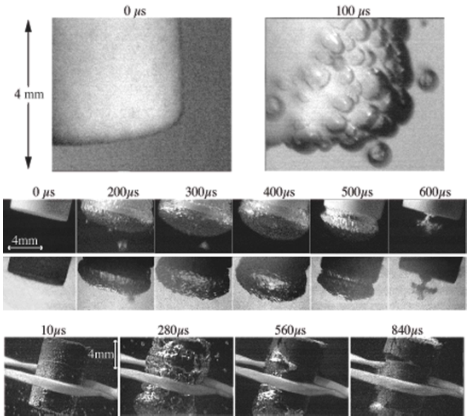
\includegraphics[width=\textwidth]{./PNGs/Cavitation.png}
		\caption{Cavitation bubble clouds. Bottom plate shows bubble activity to have forced open a crack in the stone. \cite{Bailey_2006}}
		\label{fig:cavitation}
	\end{figure}
	
	Ultrasound is perhaps best known for its use in medical imaging, where low-power ($<$ 1 W/m$^2$), high frequency ($>$ 1 MHz) ultrasound waves are used to produce high-resolutions of inhomogeneous materials, such as a fetus. Similar to SONAR or RADAR, an image can be reconstructed from reflected ultrasound waves based on time-delay, intensity, and/or frequency shift. The frequency of the wave determines the resolution of the image (with higher frequency producing better resolution), while the power of the ultrasound is kept low to prevent heating or cavitation.
	
	For surgical applications, ultrasound is used to intentionally induce the two-side effects discussed previously, heating and cavitation. Heating is used to cause lesions on tissues, such as tumors. Cavitation is used primarily to destroy hardened masses that would be unaffected by heating.
			
	\subsection{Ultrasonic Cavitation}
	
		Ultrasound is used in multiple therapeutic treatments. The most common use is lithotripsy. Lithotripsy is the process of pulverizing kidney stones, bezoars, gallstones, or other hardened masses inside a human body. Shock wave lithotripsy (SWL) is the ultrasonic variation and is a common treatment for kidney stones. However, shortly after the introduction of SWL to the United States in 1984 adverse effects began to be reported. \cite{Bailey_2006}
		
		The original lithotripter and most modern day lithotripters are single element pulsed sources. The patient is submerged in a water bath, or a gel is used to acoustically couple the ultrasound into the body. Each pulse is a 1 ${\mu}$s positive pressure spike, followed by a 4 ${\mu}$s negative pressure trough. Peak amplitudes range with from 15-150 MPa. Treatment generally administers 2000-4000 cycles at 0.5 - 2 Hz. \cite{Bailey_2006} Cavitation is intentionally caused along the surface of the stone to pulverize it. Unfortunately, all impedance mismatches in the system, i.e. any intersection of tissue fluid, has the potential to have cavitation effects form along it.	
				
	\subsection{Ultrasonic Heating}
		
		Ultrasonic heating was first used surgically in 1942 to treat neurological symptoms in dogs. Unfortunately, unwanted heating of the scalp made the treatment unsatisfactory.  To circumvent this heating, a craniectomy was performed to provide a waveguide for the ultrasound into the skull cavity.  This method was used to perform prefrontal transdural ablation, i.e. a lobotomy. Eventually, the problems surrounding the skull were bypassed altogether by switching to radiotherapy. \cite{Marquet_2013}
		
		The skull (and bones in general) present many problems for ultrasound treatments. The skull's irregular shape and nonuniform thickness make it difficult to establish a focus inside the brain cavity. Additionally, bone has a high speed of sound (2700 m/s), which leads to a very large impedance mismatch between air (343 m/s) or water (1497 m/s). This impedance mismatch greatly attenuates any signal attempting to travel into the brain cavity. In a different system, low receive power can often be overcome with increased transmit power, but transskull ultrasonics inadvertently burn the scalp with increased power. \cite{Sun_1998}
	
		The attenuation and focus scattering have been corrected by a minimally invasive technique of inserting a hydrophone before treatment to characterize and correct aberrations. \cite{Thomas_1996} However, with modern computing and modeling it should be possible to numerically predict acoustical properties without invasive techniques. Using Magnetic Resonance Imaging (MRI) or Computed Tomography (CT) scans, propagation through the skull can be simulated through a variety of methods. Once the distortions are accurately modeled, signal processing techniques such as time reversal or phase conjugation can correct aberrations. \cite{Marquet_2013}
		
		To overcome the heating of scalp, research attempted to move to lower frequency ultrasound (220 kHz), as lower frequencies penetrate the skull more easily. \cite{Sun_1998} Unfortunately, the first patient treated died five days later from serious hemorrhaging. Further human tests of transskull therapy have reported post-treatment complications. \cite{Marquet_2013}
		
\section{Current Research}
		
	In both surgical applications of ultrasound, unintended consequences are the result of impedance mismatches in the patient. As discussed in the previous section, bone, tissue, water, blood, etc. all have different speeds of sound, providing barriers where unwanted heating and cavitation can occur.  
	
	\subsection{Time Reversal Signal Processing}
	
		One technique uses Time Reversal Mirrors (TRMs) to automatically compensate for impedance mismatches. The TRM emits a plane wave which travels to a target and reflects back. The reflected signal appears to the TRM as a (weak) transmitted signal. The TRM time reverses the reflected signal $p(r,T-t)$ and retransmits. This retransmitted wave is more focused on the target. This process is repeated, with each iteration having an improved focus upon the target.  This technique can be improved by using an implanted hydrophone, but non-invasive options also work. \cite{Chakroun_1995} \cite{Thomas_1996} Figure~\ref{fig:time_reversal} shows how time reversal techniques can correct for aberrations in an inhomogeneous material.
		
				\begin{figure}[h!]
					\centering
					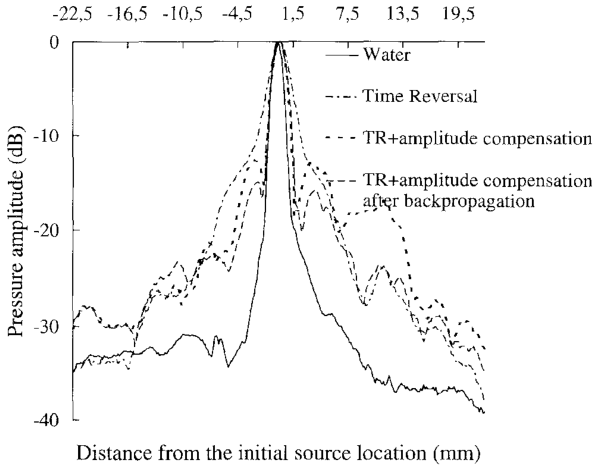
\includegraphics[width=.75\textwidth]{./PNGs/Time_Reversal.png}
					\caption{Pressure amplitude of the received signal vs. distance into the medium. \cite{Thomas_1996}}
					\label{fig:time_reversal}
				\end{figure}
	
	\subsection{Phased Array}
	
		Another technique to reduce these unintended consequences is phased array architecture. Multiple elements are arranged so the acoustic wave radiated from each source element will add up at the desired focal point, while canceling each other in the rest of the system. Figure~\ref{fig:phased_array} shows the focusing effects of increasing the number of elements in the array. Correctly aligning multiple arrays greatly reduces scattering into the sidelobes.\cite{Sun_1998}
		
		\begin{figure}[h!]
			\centering
			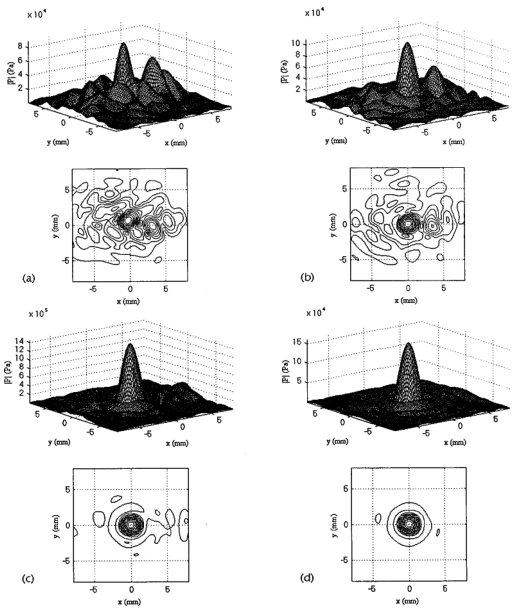
\includegraphics[width=\textwidth]{./PNGs/Phased_Array.png}
			\caption{Transskull ultrasonic field for different array combinations: (a) 1 X 1; (b) 4 X 4; (c) 8 X 8; (d) 16 X 16. \cite{Sun_1998}}
			\label{fig:phased_array}
		\end{figure}
			
		To test the phased array approach, Marquet \textit{et al.} induced brain tissue coagulation via ultrasonic heating in the brains of monkeys. This was achieved using a 1 MHz system with a tight focus. CT scans were used to target the brain tissues, while thermal doses were estimated from numerical computation. The aim of the study was to check if it was possible to induce thermal lesions 2 cm deep through the intact skull. \cite{Marquet_2013}
		
		The system Marquet \textit{et al.} used was composed of three hundred piezocomposite transducers on a spherical surface. Each transducer was capable of independent programming. A latex membrane filled with water was used to acoustically couple the ultrasound into the skull, as well as provide cooling for the surface of the skin. The signals for the transducers required a 90 minute simulation to calculate. \cite{Marquet_2013}
		
		For each targeted area, a 10-s sonication at fixed power was repeated 10 times with a 20-s cooling delay between sonications to allow the skin to cool. Each animal was first treated in the left hemisphere, woken up, and then followed up for 15 days. The procedure was then repeated in the right hemisphere, and the monkeys were kept under observation for two days before sacrifice, and the brains were preserved for examination. \cite{Marquet_2013}
		
		The cooling time between sonications was sufficient to avoid skin burns in seven of the eight experiments. The only skin burn observed was not located along the beam path, but rather at the rear of the head, at the boundary of the contact between the water balloon and the skin.  Most probably an air bubble was trapped at this location, creating a large impedance mismatch and excessive heating. This monkey was also the only subject to exhibit side effects after treatment. \cite{Marquet_2013}
		
		Interestingly, no lesions could be detected in one tissue sample despite the high estimated thermal dose. The authors suspected it could have been due to cavitation in the water-coupling balloon. Such micro-bubbles could have created an ultrasonic wall, preventing the ultrasound from entering the skull cavity. \cite{Marquet_2013}
		
		MRI control would allow the system to further refine the duration of sonication and cooling to create optimal ablation/thermal dosage.  As of the publishing, a MRI compatible prototype is under development. \cite{Marquet_2013}
		
\section{Conclusion}

	This paper explored some of the current research being done in ultrasonic surgery, specifically transskull ultrasonics. Signal processing techniques, such as time reversal, and different antennas, such as phased arrays, are two of the ways researchers are attempting to eliminate the unwanted side effects of heating and cavitation. 
	
	Marquet \textit{et al.} were able to demonstrate a non-invasive procedure for inducing thermal lesions through the skull-cavity of monkeys. Their phased array architecture requires precise instrumentation and position of the system, as well as computation time to calculate the needed vectors for the multiple sources. A time reversal technique, on the other hand, is optimized with an inserted hydrophone, but can operate without one. These methods could also be combined to take advantage of both, but would also incur some of the negatives of both.
	
\pagebreak		
\printbibliography
		
\end{document}